\documentclass[10pt,oneside,slovak,a4paper]{article}

\usepackage[slovak]{babel}

\usepackage[IL2]{fontenc} 
\usepackage[utf8]{inputenc}
\usepackage{graphicx}
\usepackage{listings}
\usepackage{verbatim}
\usepackage{url}
\usepackage{amsfonts}
\usepackage{hyperref} 
\usepackage{cite}
\usepackage[margin=1.3in]{geometry}
\usepackage{float}

\setlength{\tabcolsep}{18pt}
\renewcommand{\arraystretch}{1.5}

\lstset{literate=%
         {á}{{\'a}}1
         {í}{{\'i}}1
         {é}{{\'e}}1
         {ý}{{\'y}}1
         {ú}{{\'u}}1
         {ó}{{\'o}}1
         {ě}{{\v{e}}}1
         {š}{{\v{s}}}1
         {č}{{\v{c}}}1
         {ľ}{{\v{l}}}1
         {ř}{{\v{r}}}1
         {ž}{{\v{z}}}1
         {ď}{{\v{d}}}1
         {ť}{{\v{t}}}1
         {ň}{{\v{n}}}1                
         {ů}{{\r{u}}}1
         {Á}{{\'A}}1
         {Í}{{\'I}}1
         {É}{{\'E}}1
         {Ý}{{\'Y}}1
         {Ú}{{\'U}}1
         {Ó}{{\'O}}1
         {Ě}{{\v{E}}}1
         {Š}{{\v{S}}}1
         {Č}{{\v{C}}}1
         {Ř}{{\v{R}}}1
         {Ž}{{\v{Z}}}1
         {Ď}{{\v{D}}}1
         {Ť}{{\v{T}}}1
         {Ň}{{\v{N}}}1                
         {Ů}{{\r{U}}}1
         {Ä}{{\"A}}1
         {Ľ}{{\v{L}}}1
         {ä}{{\"a}}1    
}

\pagestyle{headings}


\begin{document}

\begin{titlepage}
	\centering
	\par\vspace{1cm}
	{\scshape\LARGE Slovenská technická univerzita v Bratislave \par}
	{\scshape\Large Fakulta informatiky a informačných technológií\par}
	\vspace{1.5cm}
	{\large Princípy informačných systémov \par}
	{\large Dokumentácia projektu\par}
	\vspace{5cm}
	{\huge\bfseries Repozitár - digitálna knižnica\par}
	\vspace{0.5cm}
	{\Large\itshape Dávid Kubík, Martin Staňo, Veronika Včelková\par}
	\vfill
	cvičiaci\par
	RNDr. Marta \textsc{Gnipová}, Ing. Nadežda \textsc{Andrejčíková}, PhD.\par
	\vspace{1cm}
	{\large \today\par}
\end{titlepage}

\tableofcontents

\newpage


\section{Percentuálny podiel práce autov na projekte}

\vspace{1cm}

\begin{tabular}{ |p{3cm}||p{2.5cm}|p{3cm}|p{2.5cm}|}
 \hline
 \multicolumn{4}{|c|}{\textbf{Podiel práce}} \\
 \hline
 Časť projektu & Dávid Kubík & Martin Staňo & Veronika Včelková\\
 \hline
 Počiatočný návrh a identifikácia úloh & 30 & 30 &  40\\
 \hline
 Zapracovanie pripomienok z konzultácií a vytvorenie návrhu v IBM BPM & 40 & 30 &  30\\
 \hline
 Návrh formulárov & 30 & 30 &  40\\
 \hline
 Návrh použitia webových služieb & 30 & 40 &  30\\
 \hline
 Implementácia v IBM BPM & 30 & 40 &  30\\
 \hline
 Vypracovanie dokumentácie & 40 & 30 &  30\\
 
 \hline
\end{tabular}

\newpage

\section{Špecifikácia projektu: Repozitár - digitálna knižnica}

\subsection{Úvod}

Cieľom tohto projektu je definovať biznis procesy na podporu nižšie popísanej problémovej domény. Tieto biznis procesy budu navrhnuté, implementované a otestované v prostredí IBM BPM. Pri návrhu a implementácií biznis procesov sa dbalo na dodržiavanie princípov SOA (využívanie webových služieb a ich správne prepojenie).


\subsection{Špecifikácia}

Horizont H2020 určuje vedeckovýskumným pracoviskám povinnosť evidovať svoje publikované výsledky VaV v repozitári – vlastnom, konzorcionálnom, národnom. Údaje, ktoré popisujú dokument – bibliografický záznam, môže vykonávať spracovateľ, knihovník, alebo priamo vedec.

Formulár obsahuje minimálne všetky základné údaje nevyhnutné pre jednoznačnú identifikáciu daného typu dokumentu. Pri vkladaní dát sú priebežne systémom vykonávané viaceré kontroly, dôležité je, aby všetky entity boli identifikovaný perzistentným jedno-jednoznačným identifikátorom, teda aby v systéme nemohli na základe termínu reprezentujúceho dané idivídum vznikať homonymá, ale zároveň aby systém vedel k danému termínu agregovať všetky jeho synonymá, akronymy, či iné variantné formy termínov, ktoré môžu vystihovať význam tohto indivídua.

Zadané údaje sa vždy uložia do systému aj s prípadnými chybami, všetky údaje sú logované a v prípade, že neexistuje identifikátor pre dané indivídum entity, systém vytvorí nový záznam pre toto individum a pridelí mu požadovaný identifikátor a následne vo formulári prelinkuje na tento identifikátor.

Všetky vzťahy medzi entitami sú evidované na základe významu a prostredníctvom uvedených identifikátorov, teda nie odkaz na termín, ten sa generuje následne prostredníctvom daného identifikátora z príslušnej databázy modelu. 

Konečnú platnosť a správnosť údajov, môže potvrdiť až knihovník, vtedy sa všetky údaje pre iný používateľov a teda aj autorov stávajú len read/only, návrh na akúkoľvek zmenu môžu vykonať len prostredníctvom mailu, alebo poznámky k záznamu. Ak údaje vkladá spracovateľ, alebo vedecký pracovník, ostatní spoluautori ako aj konkrétny spracovateľ sú o tom informovaní , rovnako ako aj v prípade, keď knihovník potvrdí správnosť a zverejní záznam. 

Samozrejme autori určujú podmienky, pre koho bude záznam aj dokument dostupný voľne a pre ktoré skupiny na vyžiadanie, prípadne pre koho zasa úplne neviditeľný, pričom môže toto kombinovať aj s časovým určením, teda napr. pre pracovníkov oddelenia voľne dostupný pre ostatných akademických a vedecko-pedagogických pracovníkov voľne dostupný po 2 rokoch a pre ostatných viditeľný po 3 a voľne dostupný po 5 rokoch.

Navrhnite procesy, ktoré umožnia spracovať a sprístupňovať repozitár publikovaných výsledkov vedy a výskumu tak, že bude zároveň evidovať všetky vzájomné vzťahy medzi entitami použitými pre popis publikovaného výsledku VaV na základe významu.

\newpage

\subsection{Vypracovanie projektu}
Návrh aj implementácia nášho projektu bude realizovaná vo vývojovom prostredí IBM Business Process Designer 8.5.5. Diagram dátového modelu bude vytvorený vo webovom nástroji draw.io.


\section{Návrh, analýza a opis biznis procesov}

V tomto projekte budú analyzované a implementované nasledujúce biznis procesy súvisiace s problémovou doménou:

\begin{itemize}
\item nahranie digitálneho objektu pre bibliografický záznam,
\item validácia digitálneho objektu,
\item nahranie bibliografického záznamu.
\end{itemize}

\newpage

\subsection{Dátový model}
Vo vyššie pomenovaných biznis procesoch sme identifikovali nasledujúce entity ako aj ich atribúty a vzťahy medzi nimi. Tieto entity zároveň reprezentujú naše biznis objekty (komplexné dátové typy).

\begin{figure} [H]
\label{datamodel}
\centering
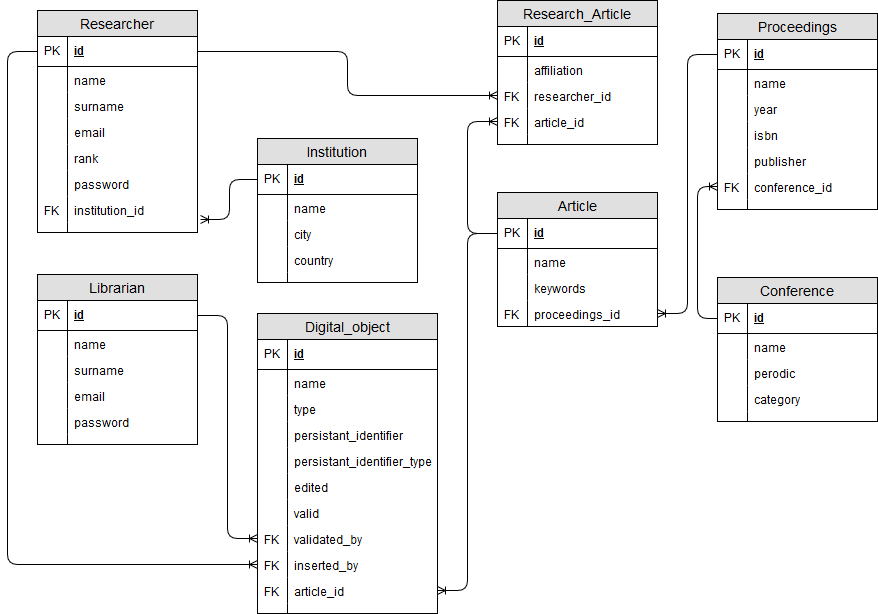
\includegraphics[scale=0.4]{datovy_model.png} 
\caption{ER diagram dátového modelu}
\end{figure}

\subsection{Main Business Process}
V nasledujúcich podkapitolách sa bližšie pozrieme na hlavný biznis proces.

\subsubsection{Cieľ biznis procesu}
Cieľom tohto biznis procesu je integrácia všetkej funkcionality poskytovanej systémom. Jednotlivé funkcionality sú integrované ako podprocesy tohto hlavného procesu.

\subsubsection{Používateľské roly}
Jednotlivé kroky procesu sú rozdelené vo viacerých plaveckých dráhach, ktoré predstavujú dva samostatné systémy.

\begin{itemize}
\item \textbf{Systém} Táto plavecká dráha obsahuje úlohy, ktoré bude vykonávať nami navrhovaný systém.
\item \textbf{Používateľ} Táto plavecká dráha obsahuje úlohy, ktoré bude vykonávať používateľ systému. Používateľom, môže byť spracovateľ, knihovník, alebo vedec.
\item \textbf{Knihovník} Táto plavecká dráha obsahuje úlohy, ktoré bude vykonávať knihovník.
\end{itemize}

\newpage

\subsubsection{Biznis objekty}
\textbf{Institution}\\
Tento biznis objekt reprezentuje vedeckovýskumné pracovisko, ktoré eviduje publikované výsledky v digitálnom repozitári. Parametre tohto biznis objektu sú nasledovné:

\begin{itemize}
\item \textbf{id:} unikátny primárny kľúč v systémovej databáze,
\item \textbf{name:} názov inštitúcie, pod ktorým je registrovaná v obchodnom registri Slovenskej republiky,
\item \textbf{city:} mesto, v ktorom má daná inštitúcia hlavné sídlo,
\item \textbf{country:} krajina, v ktorom je hlavné sídlo danej inštitúcie.
\end{itemize}

\textbf{Librarian}\\
Tento biznis objekt reprezentuje knihovníka digitálneho repozitáru, ktorý má na starosti okrem iného aj potvrdzovanie správnosti zadaných údajov digitálneho objektu bibliografického záznamu. Parametre tohto biznis objektu sú nasledovné:

\begin{itemize}
\item \textbf{id:} unikátny primárny kľúč v systémovej databáze,
\item \textbf{name:} krstné meno uvedené v rodnom liste pracovníka vedeckovýskumného ústavu,
\item \textbf{surname:} priezvisko uvedené v rodnom liste pracovníka vedeckovýskumného ústavu,
\item \textbf{email:} emailová schránka pracovníka vedeckovýskumného ústavu,
\item \textbf{password:} prístupové heslo do systému.
\end{itemize}

\textbf{Researcher}\\
Tento biznis objekt reprezentuje zamestnanca vedeckovýskumného pracoviska, ktorý svoje výsledky publikuje do digitálneho repozitára. Parametre tohto biznis objektu sú nasledovné:

\begin{itemize}
\item \textbf{id:} unikátny primárny kľúč v systémovej databáze,
\item \textbf{name:} krstné meno uvedené v rodnom liste pracovníka vedeckovýskumného ústavu,
\item \textbf{surname:} priezvisko uvedené v rodnom liste pracovníka vedeckovýskumného ústavu,
\item \textbf{email:} emailová schránka pracovníka vedeckovýskumného ústavu,
\item \textbf{rank:} úroveň pracovníka k sprístupneniu publikácií,
\item \textbf{password:} prístupové heslo do systému,
\item \textbf{institution\_id:} cudzí kľúč v systémovej databáze, ktorý sa odkazuje na konkrétnu inštitúciu,
\item \textbf{phone:} telefónne číslo.
\end{itemize}

\textbf{Research\_Article}\\
Tento biznis objekt reprezentuje prepojovaciu tabuľku v systémovej databáze medzi vedcami a publikáciami. K tomuto kroku sme pristúpili z dôvodu, aby sme vedeli korektne vyjadriť vzťah many-to-many. Parametre tohto biznis objektu sú nasledovné:

\begin{itemize}
\item \textbf{id:} unikátny primárny kľúč v systémovej databáze,
\item \textbf{affilation:} rola autora/spoluautora na danom bibliografickom zázname, napr. spoluautor, prekladateľ, ilustrátor,
\item \textbf{researcher\_id:} cudzí kľúč v systémovej databáze, ktorý sa odkazuje na autora publikovaného bibliografického záznamu v digitálnom repozitári,
\item \textbf{article\_id:} cudzí kľúč v systémovej databáze, ktorý sa odkazuje na publikovaný bibliografický záznam v digitálnom repozitári,
\item \textbf{work\_share:} podiel práce.
\end{itemize}

\textbf{Proceedings}\\
Tento biznis objekt reprezentuje zborník, ktorý vznikol ako dôsledok určitej vedeckej konferencie. Parametre tohto biznis objektu sú nasledovné:

\begin{itemize}
\item \textbf{id:} unikátny primárny kľúč v systémovej databáze,
\item \textbf{name:} názov zborníku vedeckej konferencie,
\item \textbf{year:} rok, kedy bol zborník vedeckej konferencie vydaný,
\item \textbf{isbn:} medzinárodné štandardné číslo knihy (z angl. international standard book number) pod ktorým bol zborník vedeckej konferencie publikovaný,
\item \textbf{publisher:} vydavateľ zborníku vedeckej konferencie,
\item, \textbf{conference\_id:} cudzí kľúč v systémovej databáze, ktorý sa odkazuje na vedeckú konferenciu.
\end{itemize}

\textbf{Article}\\
Tento biznis objekt reprezentuje bibliografický záznam v databáze vedeckovýskumného pracoviska. Parametre tohto biznis objektu sú nasledovné:

\begin{itemize}
\item \textbf{id:} unikátny primárny kľúč v systémovej databáze,
\item \textbf{name:} názov publikácie, pod ktorým je uvedená v databáze vedeckovýskumného pracoviska,
\item \textbf{keywords:} kľúčové slová, ktoré sa využívajú pri vyhľadaní danej publikácie v digitálnom repozitári,
\item \textbf{proceedings\_id:} cudzí kľúč v systémovej databáze, ktorý sa odkazuje na zborník vedeckej konferencie.
\end{itemize}

\textbf{Conference}\\
Tento biznis objekt reprezentuje vedeckú konferenciu. Parametre tohto biznis objektu sú nasledovné:

\begin{itemize}
\item \textbf{id:} unikátny primárny kľúč v systémovej databáze,
\item \textbf{name:} názov vedeckej konferencie,
\item \textbf{periodic:} vyjadruje pravdivostnú hodnotu periodicity vedeckej konferencie, či sa opakuje v pravidelných intervaloch,
\item \textbf{category:} oblasť výskumu vedeckej konferencie,
\item \textbf{calendar\_year:} kalendárny rok konania vedeckej konferencie,
\item \textbf{conference\_year:} ročník konania vedeckej konferencie,
\item \textbf{from\_date:} dátum začatia daného ročníka vedeckej konferencie,
\item \textbf{to\_date:} dátum ukončenia daného ročníka vedeckej konferencie.
\end{itemize}

\textbf{Digital\_object}\\
Tento biznis objekt reprezentuje digitálny objekt uložený v digitálnom repozitári. Parametre tohto biznis objektu sú nasledovné:

\begin{itemize}
\item \textbf{id:} unikátny primárny kľúč v systémovej databáze,
\item \textbf{name:} názov digitálneho objektu v digitálnom repozitári,
\item \textbf{type:} typ digitálneho objektu, napr. abstrakt, plný text,
\item \textbf{persistent\_identifier:} perzistentný identifikátor, cez ktorý je digitálny objekt prístupná na internete,
\item \textbf{persistent\_identifier\_type:} typ perzistnentného identifikátoru, napr. doi, ark, eisp,
\item \textbf{edited:} dátum poslednej úpravy digitálneho objektu,
\item \textbf{valid:} pravdivostná hodnota vyjadrujúca, či zadané údaje v digitálnom objekte sú korektné,
\item \textbf{validated\_by:} cudzí kľúč v systémovej databáze, ktorý sa odkazuje na zamestnanca, ktorý kontroloval správnosť údajov digitálneho objektu,
\item \textbf{inserted\_by:} cudzí kľúč v systémovej databáze, ktorý sa odkazuje na zamestnanca, ktorý vložil digitálny objekt do digitálneho repozitáru,
\item \textbf{article\_id:} cudzí kľúč v systémovej databáze, ktorý sa odkazuje na bibliografický záznam, z ktorého bol digitálny objekt vytvorený,
\item \textbf{inserted\_date:} dátum vloženia digitálneho objektu do databázy,
\item \textbf{validated\_date:} dátum validácie správnosti údajov digitálneho objektu.
\end{itemize} 

\textbf{Event}\\
Tento biznis objekt reprezentuje logovací záznam. Parametre tohto biznis objektu sú nasledovné:

\begin{itemize}
\item \textbf{id:} unikátny primárny kľúč v systémovej databáze,
\item \textbf{timestamp:} dátum a čas, kedy vznikol logovací záznam,
\item \textbf{message:} správa, ktorá sa má zalogovať,
\item \textbf{severity:} závažnosť (Info, Warning, Error).
\end{itemize}

\section{Implementácia systémových úloh}
\paragraph{Biznis proces - Hlavný biznis proces}
\textbf{Rola:} Super User, Vedec, Systém, Knihovník\\
\textbf{Výstup:}

\begin{itemize}
\item \textbf{finished} - pravdivostná hodnota, či biznis proces skončil
\end{itemize}

Používateľ zadá svoje prihlasovacie údaje. Systém overí správnosť týchto údajov a v prípade správnych prihlasovacích údajov, prihlási používateľa ako knihovníka.

\begin{figure} [H]
\centering
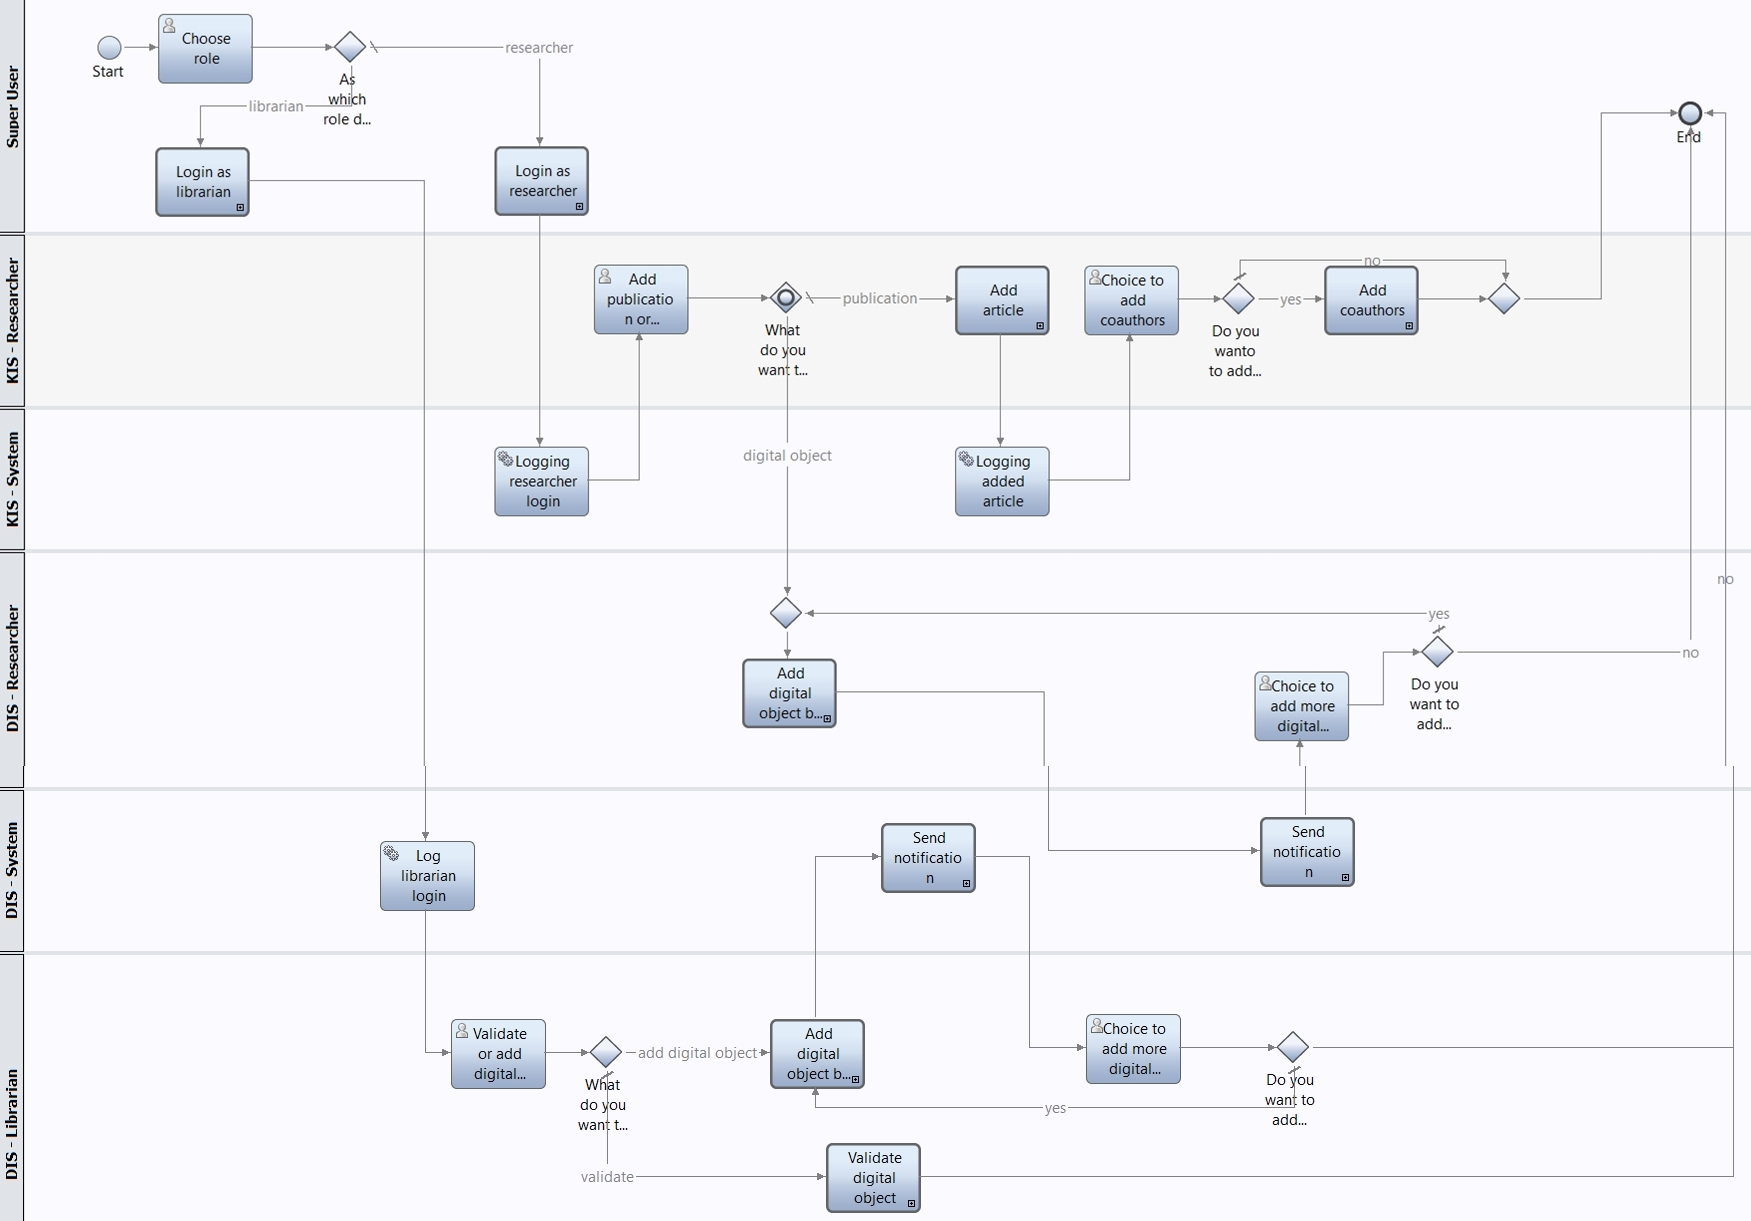
\includegraphics[scale=0.35]{diagrams/diagUpload.jpg} 
\caption{Diagram hlavného biznis procesu}
\end{figure}

Predstavuje hlavný biznis proces, ktorý sa skladá z mnoho podprocesov, ktoré vykonávajú samotnú funkcionalitu systému. Hlavný biznis proces zobrazuje dva systémy, ktoré spolupracujú na splnení biznis procesu a jeho cieľov. Na samostatné funkcionality systému sa pozrieme v nasledovných podkapitolách:

\subsection{Login as Librarian - používateľská úloha}
\textbf{Rola:} Knihovník\\
\textbf{Výstup:}

\begin{itemize}
\item \textbf{librarian} - objekt typu Librarian
\end{itemize}

Používateľ zadá svoje prihlasovacie údaje. Systém overí správnosť týchto údajov a v prípade správnych prihlasovacích údajov, prihlási používateľa ako knihovníka.

\begin{figure} [H]
\centering
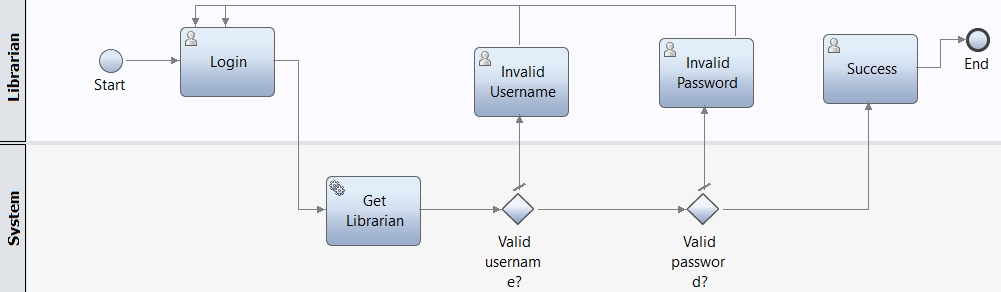
\includegraphics[scale=0.4]{diagrams/diagLoginLibrarian.jpg} 
\caption{Diagram podprocesu prihlásenia ako knihovník}
\end{figure}

\subsubsection{Webová služba: Získanie knihovníka}
\textbf{Názov služby:} WS\_Librarian\_find\\
\textbf{Metóda služby:} getById\\
\textbf{Vstupy:}
	\begin{itemize}
		\item \textit{id} - ID knihovníka
	\end{itemize}
\textbf{Výstupy:}
	\begin{itemize}
		\item \textit{librarian} - objekt typu Librarian
	\end{itemize}
	
\subsection{Login as Researcher - používateľská úloha}
\textbf{Rola:} Vedec\\
\textbf{Výstup:}

\begin{itemize}
\item \textbf{researcher} - objekt typu Researcher
\end{itemize}

Používateľ zadá svoje prihlasovacie údaje. Systém overí správnosť týchto údajov a v prípade správnych prihlasovacích údajov, prihlási používateľa ako vedca.

\begin{figure} [H]
\centering
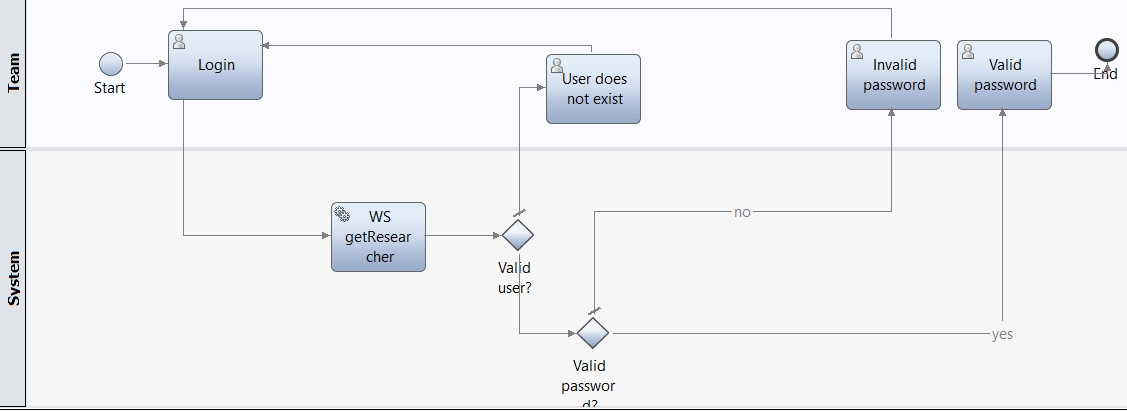
\includegraphics[scale=0.4]{diagrams/diagLoginResearcher.jpg} 
\caption{Diagram podprocesu prihlásenia ako vedec}
\end{figure}

\subsubsection{Webová služba: Získanie vedca}
\textbf{Názov služby:} WS\_Researcher\_find\\
\textbf{Metóda služby:} getById\\
\textbf{Vstupy:}
	\begin{itemize}
		\item \textit{id} - ID vedca
	\end{itemize}
\textbf{Výstupy:}
	\begin{itemize}
		\item \textit{researcher} - objekt typu Researcher
	\end{itemize}

\subsection{Add coauthors - používateľská úloha}
\textbf{Rola:} Vedec\\
\textbf{Vstup:}

\begin{itemize}
\item \textbf{article\_id} - Integer hodnota reprezentujúca ID článku
\end{itemize}

Používateľ si vyberie článok, ku ktorému chce pridať spoluautorov a následne si buď vyberie zo zoznamu spoluautora, alebo ak v tomto zozname nie je, tak zadá údaje spoluautora manuálne.

\begin{figure} [H]
\centering
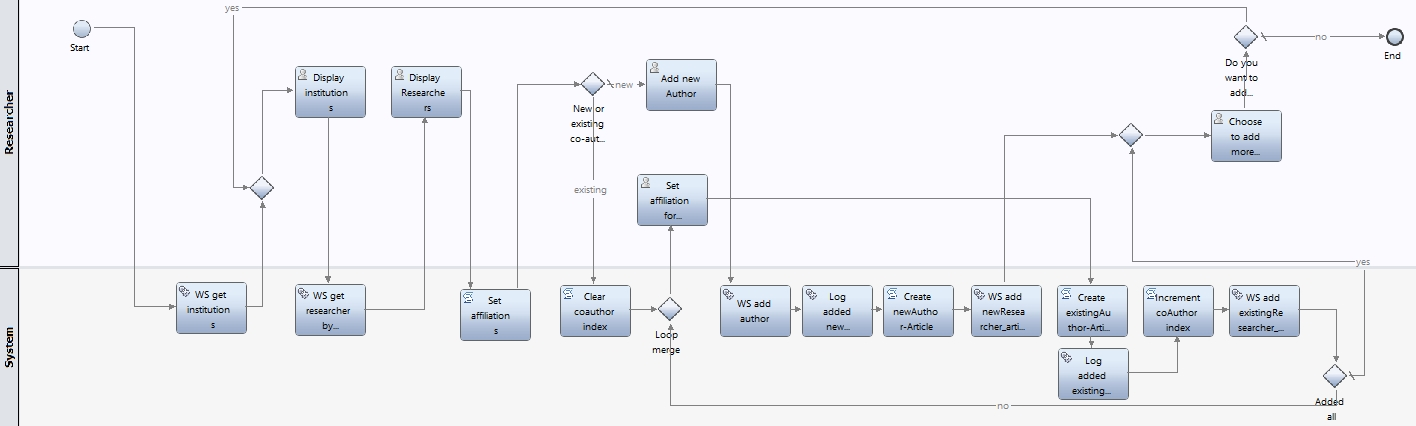
\includegraphics[scale=0.4]{diagrams/diagAddCoauthors.jpg} 
\caption{Diagram podprocesu pridania spoluautorov}
\end{figure}

\subsubsection{Webová služba: Získanie všetkých inštitúcií}
\textbf{Názov služby:} WS\_Institution\_findAll\\
\textbf{Metóda služby:} getAll\\
\textbf{Výstupy:}
	\begin{itemize}
		\item \textit{institutions} - list objektov typu Institution
	\end{itemize}
	
\subsubsection{Webová služba: Získaj vedca podľa ľubovoľného atribútu}
\textbf{Názov služby:} WS\_Researcher\_getByAttribute\\
\textbf{Metóda služby:} getByAttributeValue\\
\textbf{Vstupy:}
	\begin{itemize}
		\item \textit{name} - názov atribútu, podľa ktorého sa má vyhľadávať
		\item \textit{value} - hodnota atribútu, podľa ktorého sa má vyhľadávať
		\item \textit{listOf.Integer()} - zoznam ID vedcov, z ktorých sa má hľadať, vytvárame nový prázdny list, aby metóda služby hľadala v celom rozsahu (všetkých IDs)
	\end{itemize}
\textbf{Výstupy:}
	\begin{itemize}
		\item \textit{researchers} - list objektov typu Researcher 
	\end{itemize}
	
\subsubsection{Skript: Nastav afiláciu}
Skript na naplnenie pola na data do grafickeho rozhrania ku radio buttonom.

\subsubsection{Skript: Vynuluj index spoluautorov}
Skript, ktorý nastaví index na nulu. Je to potrebné kvôli cykleniu.

\subsubsection{Webová služba: Vloženie vedca}
\textbf{Názov služby:} WS\_Reasercher\_insert\\
\textbf{Metóda služby:} insert\\
\textbf{Vstupy:}
	\begin{itemize}
		\item \textit{team\_id} - ID tímu, slúži na autentifikáciu webovej služby
		\item \textit{team\_password} - heslo, slúži na autentifikáciu webovej služby
		\item \textit{researcher} - objekt typu Researcher s vyplnenými údajmi
	\end{itemize}
\textbf{Výstupy:}
	\begin{itemize}
		\item \textit{id} - ID novo vytvoreného vedca
	\end{itemize}

\subsubsection{Webová služba: Vloženie logovacieho záznamu}
\textbf{Názov služby:} WS\_Events\_insert\\
\textbf{Metóda služby:} insert\\
\textbf{Vstupy:}
	\begin{itemize}
		\item \textit{team\_id} - ID tímu, slúži na autentifikáciu webovej služby
		\item \textit{team\_password} - heslo, slúži na autentifikáciu webovej služby
		\item \textit{event} - objekt typu Events vyplnenými údajmi
	\end{itemize}
\textbf{Výstupy:}
	\begin{itemize}
		\item \textit{id} - ID novo vytvoreného logovacieho záznamu
	\end{itemize}
	
\subsubsection{Skript: Pridaj nového spoluautora ku vedeckej publikácii}
Skript na vytvorenie nového objektu, ktorý priradí nového spoluautora k danej vedeckej publikácii. Potom tento objekt pridá webová služba do prepojovacej tabuľky Researcher\_Article.

\subsubsection{Webová služba: Vloženie entity spojovacej tabuľky Vedec - Publikácia}
\textbf{Názov služby:} WS\_Researcher\_article\_insert\\
\textbf{Metóda služby:} insert\\
\textbf{Vstupy:}
	\begin{itemize}
		\item \textit{team\_id} - ID tímu, slúži na autentifikáciu webovej služby
		\item \textit{team\_password} - heslo, slúži na autentifikáciu webovej služby
		\item \textit{researcher\_article} - objekt typu Researcher\_Article s vyplnenými údajmi
	\end{itemize}
\textbf{Výstupy:}
	\begin{itemize}
		\item \textit{id} - ID novo vytvorenej entity spojovacej tabuľky Vedec - Publikácia
	\end{itemize}
	
\subsubsection{Skript: Pridaj existujúceho spoluautora ku vedeckej publikácii}
Vytvorí objekt do prepojovacej tabuľky. Existujúceho autora priradí k danej vedeckej publikácii.

\subsubsection{Skript: Inkrementuj index spoluautorov}
Skript na inkrementovanie indexu spoluautorov. Je potrebný pre správne fungovanie cyklu.

\subsection{Add digital object by Researcher - používateľská úloha}
\textbf{Rola:} Vedec\\
\textbf{Vstup:}

\begin{itemize}
\item \textbf{logged\_researcher} - objekt typu Researcher
\end{itemize}

\textbf{Výstup:}

\begin{itemize}
\item \textbf{chosen\_article} - objekt typu Article
\end{itemize}

Používateľ si vyberie konferenciu, zborník a napokon konkrétnu vedeckú publikáciu. Následne k tomuto článku priradí digitálny objekt.

\begin{figure} [H]
\centering
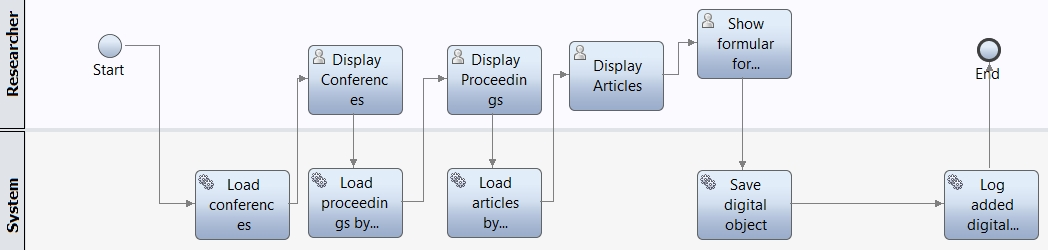
\includegraphics[scale=0.4]{diagrams/diagAddDigital.jpg} 
\caption{Diagram podprocesu pridávania digitálnych objektov vedcom}
\end{figure}

\subsubsection{Webová služba: Získanie vedeckých publikácií na základe atribútu}
\textbf{Názov služby:} WS\_Article\_getByAttribute\\
\textbf{Metóda služby:} getByAttributeValue\\
\textbf{Vstupy:}
	\begin{itemize}
		\item \textit{attributes\_name} - názov atribútu
		\item \textit{attributes\_value} - hodnota atribútu
		\item \textit{listOf.Integer()} - zoznam ID vedeckých publikácií, z ktorých sa má hľadať, vytvárame nový prázdny list, aby metóda služby hľadala v celom rozsahu (všetkých IDs)
	\end{itemize}
\textbf{Výstupy:}
	\begin{itemize}
		\item \textit{articles} - list objektov typu Article
	\end{itemize}

\subsubsection{Webová služba: Získanie všetkých vedeckých konferencií}
\textbf{Názov služby:} WS\_Conference\_findAll\\
\textbf{Metóda služby:} getAll\\
\textbf{Výstupy:}
	\begin{itemize}
		\item \textit{conferences} - list objektov typu Conference
	\end{itemize}
	
\subsubsection{Webová služba: Získanie zborníka podľa ľubovoľného atribútu}
\textbf{Názov služby:} WS\_Proceedings\_getByAttribute\\
\textbf{Metóda služby:} getByAttributeValue\\
\textbf{Vstupy:}
	\begin{itemize}
		\item \textit{attributes\_name} - názov atribútu
		\item \textit{attributes\_value} - hodnota atribútu
		\item \textit{listOf.Integer()} - zoznam ID zborníkov, z ktorých sa má hľadať, vytvárame nový prázdny list, aby metóda služby hľadala v celom rozsahu (všetkých IDs)
	\end{itemize}
\textbf{Výstupy:}
	\begin{itemize}
		\item \textit{proceedings} - list objektov typu Proceeding
	\end{itemize}
	
\subsubsection{Webová služba: Vloženie digitálneho objektu}
\textbf{Názov služby:} WS\_Digital\_object\_insert\\
\textbf{Metóda služby:} insert\\
\textbf{Vstupy:}
	\begin{itemize}
		\item \textit{team\_id} - ID tímu, slúži na autentifikáciu webovej služby
		\item \textit{team\_password} - heslo, slúži na autentifikáciu webovej služby
		\item \textit{digital\_object} - objekt typu Digital\_object s vyplnenými údajmi
	\end{itemize}
\textbf{Výstupy:}
	\begin{itemize}
		\item \textit{id} - ID novo vytvoreného digitálneho objektu
	\end{itemize}
	
\subsubsection{Webová služba: Vloženie logovacieho záznamu}
\textbf{Názov služby:} WS\_Events\_insert\\
\textbf{Metóda služby:} insert\\
\textbf{Vstupy:}
	\begin{itemize}
		\item \textit{team\_id} - ID tímu, slúži na autentifikáciu webovej služby
		\item \textit{team\_password} - heslo, slúži na autentifikáciu webovej služby
		\item \textit{event} - objekt typu Events vyplnenými údajmi
	\end{itemize}
\textbf{Výstupy:}
	\begin{itemize}
		\item \textit{id} - ID novo vytvoreného logovacieho záznamu
	\end{itemize}

\subsection{Send notification - systémová úloha}
\textbf{Rola:} Systém\\
\textbf{Vstup:}

\begin{itemize}
\item \textbf{article} - objekt typu Article
\end{itemize}

Systém získa všetky entity prepojovacej tabuľky Article-Researcher. Vyfiltruje tie záznamy, ktoré zodpovedajú konkrétnemu článku. Pre každý vyfiltrovaný záznam získa vedca a tomu pošle notifikáciu. Toto sa deje v cykle Vedec je notifikovaný email-om a prostredníctvo telefonického hovoru.

\begin{figure} [H]
\centering
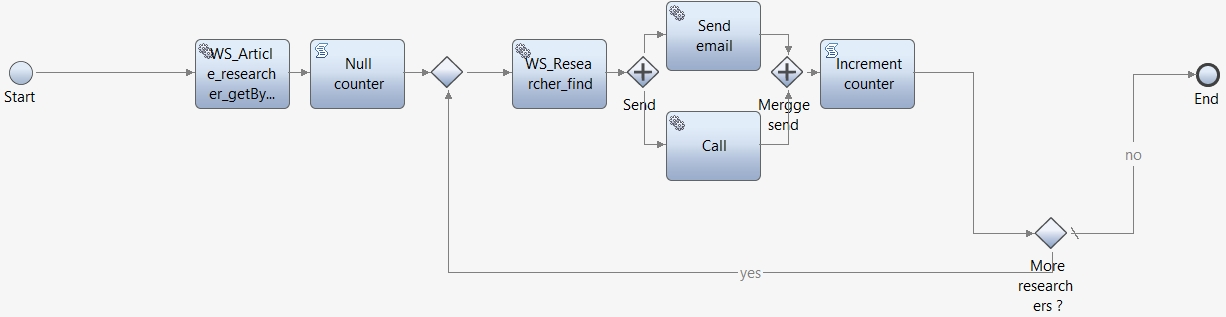
\includegraphics[scale=0.4]{diagrams/diagNotification.jpg} 
\caption{Diagram podprocesu poslania notifikácií}
\end{figure}

\subsubsection{Webová služba: Získanie vedeckých publikácií na základe atribútu}
\textbf{Názov služby:} WS\_Article\_getByAttribute\\
\textbf{Metóda služby:} getByAttributeValue\\
\textbf{Vstupy:}
	\begin{itemize}
		\item \textit{attributes\_name} - názov atribútu
		\item \textit{attributes\_value} - hodnota atribútu
		\item \textit{listOf.Integer()} - zoznam ID vedeckých publikácií, z ktorých sa má hľadať, vytvárame nový prázdny list, aby metóda služby hľadala v celom rozsahu (všetkých IDs)
	\end{itemize}
\textbf{Výstupy:}
	\begin{itemize}
		\item \textit{articles} - list objektov typu Article
	\end{itemize}

\subsubsection{Skript: Null counter}
Vynuluje počítadlo autorov vedeckej publikácie. Tento skript je potrebný pre správne fungovanie cyklu pre poslanie emailovej a telefonickej notifikácie všetkým spoluautorom.

\subsubsection{Webová služba: Získanie vedca}
\textbf{Názov služby:} WS\_Researcher\_find\\
\textbf{Metóda služby:} getById\\
\textbf{Vstupy:}
	\begin{itemize}
		\item \textit{id} - ID vedca
	\end{itemize}
\textbf{Výstupy:}
	\begin{itemize}
		\item \textit{researcher} - objekt typu Researcher
	\end{itemize}

\subsubsection{Webová služba: Poslanie emailovej notifikácie}
\textbf{Názov služby:} WS\_Send\_email\\
\textbf{Metóda služby:} notify\\
\textbf{Vstupy:}
	\begin{itemize}
		\item \textit{team\_id} - ID tímu, slúži na autentifikáciu webovej služby
		\item \textit{team\_password} - heslo, slúži na autentifikáciu webovej služby
		\item \textit{email} - emailová adresa príjemcu notifikácie
		\item \textit{"You were added as a coauthor"} - predmet správy, ktorá sa odošle
		\item \textit{"Coauthor of article: " + tw.local.article\_id.toString()} - správa, ktorá sa odošle, kde article\_id.toString() predstavuje ID článku, ktorého je príjemca spoluautorom
	\end{itemize}
\textbf{Výstupy:}
	\begin{itemize}
		\item \textit{success} - pravdivostná hodnota, ktorá vyjadruje, či sa email podarilo odoslať
	\end{itemize}

\subsubsection{Webová služba: Telefonické notifikovanie}
\textbf{Názov služby:} WS\_Call\\
\textbf{Metóda služby:} notify\\
\textbf{Vstupy:}
	\begin{itemize}
		\item \textit{team\_id} - ID tímu, slúži na autentifikáciu webovej služby
		\item \textit{team\_password} - heslo, slúži na autentifikáciu webovej služby
		\item \textit{phone} - telefónne číslo, na ktoré sa má zatelefonovať
		\item \textit{"You were added as a coauthor"} - predmet správy, ktorá sa odošle
		\item \textit{"You are coauthor of article: " + tw.local.article\_id.toString()} - správa, ktorá sa telefonicky oznámi, kde article\_id.toString() predstavuje ID článku, ktorého je príjemca telefonátu spoluautorom
	\end{itemize}
\textbf{Výstupy:}
	\begin{itemize}
		\item \textit{success} - pravdivostná hodnota, ktorá vyjadruje, či sa podarilo telefonicky notifikovať spoluautora vedeckej publikácie
	\end{itemize}

\subsubsection{Skript: Increment counter}
Zvýši počítadlo autorov vedeckej publikácie o jedna. Tento skript je potrebný pre správne fungovanie cyklu pre poslanie emailovej a telefonickej notifikácie všetkým spoluautorom.

\subsection{Add digital object by Librarian - používateľská úloha}
\textbf{Rola:} Knihovník\\
\textbf{Vstup:}

\begin{itemize}
\item \textbf{logged\_librarian} - objekt typu Librarian
\end{itemize}

\textbf{Výstup:}

\begin{itemize}
\item \textbf{chosen\_article} - objekt typu Article
\end{itemize}

Používateľ si vyberie konferenciu, zborník a napokon konkrétnu vedeckú publikáciu. Následne k tomuto článku priradí digitálny objekt.

\begin{figure} [H]
\centering
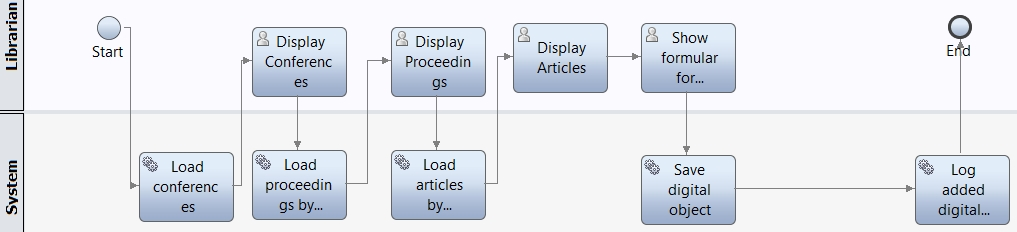
\includegraphics[scale=0.4]{diagrams/diagAddDigitalLib.jpg} 
\caption{Diagram podprocesu pridávania digitálnych objektov knihovníkom}
\end{figure}

\subsubsection{Webová služba: Získanie vedeckých publikácií na základe atribútu}
\textbf{Názov služby:} WS\_Article\_getByAttribute\\
\textbf{Metóda služby:} getByAttributeValue\\
\textbf{Vstupy:}
	\begin{itemize}
		\item \textit{attributes\_name} - názov atribútu
		\item \textit{attributes\_value} - hodnota atribútu
		\item \textit{listOf.Integer()} - zoznam ID vedeckých publikácií, z ktorých sa má hľadať, vytvárame nový prázdny list, aby metóda služby hľadala v celom rozsahu (všetkých IDs)
	\end{itemize}
\textbf{Výstupy:}
	\begin{itemize}
		\item \textit{articles} - list objektov typu Article
	\end{itemize}

\subsubsection{Webová služba: Získanie všetkých vedeckých konferencií}
\textbf{Názov služby:} WS\_Conference\_findAll\\
\textbf{Metóda služby:} getAll\\
\textbf{Výstupy:}
	\begin{itemize}
		\item \textit{conferences} - list objektov typu Conference
	\end{itemize}
	
\subsubsection{Webová služba: Získanie zborníka podľa ľubovoľného atribútu}
\textbf{Názov služby:} WS\_Proceedings\_getByAttribute\\
\textbf{Metóda služby:} getByAttributeValue\\
\textbf{Vstupy:}
	\begin{itemize}
		\item \textit{attributes\_name} - názov atribútu
		\item \textit{attributes\_value} - hodnota atribútu
		\item \textit{listOf.Integer()} - zoznam ID zborníkov, z ktorých sa má hľadať, vytvárame nový prázdny list, aby metóda služby hľadala v celom rozsahu (všetkých IDs)
	\end{itemize}
\textbf{Výstupy:}
	\begin{itemize}
		\item \textit{proceedings} - list objektov typu Proceeding
	\end{itemize}
	
\subsubsection{Webová služba: Vloženie digitálneho objektu}
\textbf{Názov služby:} WS\_Digital\_object\_insert\\
\textbf{Metóda služby:} insert\\
\textbf{Vstupy:}
	\begin{itemize}
		\item \textit{team\_id} - ID tímu, slúži na autentifikáciu webovej služby
		\item \textit{team\_password} - heslo, slúži na autentifikáciu webovej služby
		\item \textit{digital\_object} - objekt typu Digital\_object s vyplnenými údajmi
	\end{itemize}
\textbf{Výstupy:}
	\begin{itemize}
		\item \textit{id} - ID novo vytvoreného digitálneho objektu
	\end{itemize}
	
\subsubsection{Webová služba: Vloženie logovacieho záznamu}
\textbf{Názov služby:} WS\_Events\_insert\\
\textbf{Metóda služby:} insert\\
\textbf{Vstupy:}
	\begin{itemize}
		\item \textit{team\_id} - ID tímu, slúži na autentifikáciu webovej služby
		\item \textit{team\_password} - heslo, slúži na autentifikáciu webovej služby
		\item \textit{event} - objekt typu Events vyplnenými údajmi
	\end{itemize}
\textbf{Výstupy:}
	\begin{itemize}
		\item \textit{id} - ID novo vytvoreného logovacieho záznamu
	\end{itemize}
	
\subsection{Validate digital object - používateľská úloha}
\textbf{Rola:} Knihovník\\
\textbf{Vstup:}

\begin{itemize}
\item \textbf{librarian} - objekt typu Librarian
\end{itemize}

Používateľ vyberie konferenciu, zborník, a článok, pre ktorý sa načítajú digitálne objekty. Používateľ môže validovať viacero digitálnych objektov v cykle.

\begin{figure} [H]
\centering
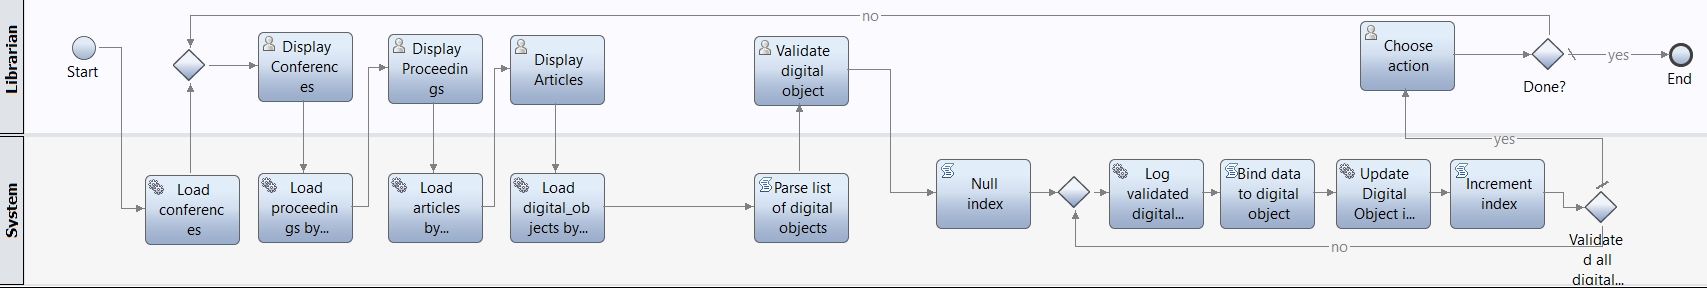
\includegraphics[scale=0.4]{diagrams/diagValidate.jpg} 
\caption{Diagram podprocesu validovania digitálneho objektu}
\end{figure}

\subsubsection{Webová služba: Získanie všetkých vedeckých konferencií}
\textbf{Názov služby:} WS\_Conference\_findAll\\
\textbf{Metóda služby:} getAll\\
\textbf{Výstupy:}
	\begin{itemize}
		\item \textit{conferences} - list objektov typu Conference
	\end{itemize}
	
\subsubsection{Webová služba: Získanie zborníka podľa ľubovoľného atribútu}
\textbf{Názov služby:} WS\_Proceedings\_getByAttribute\\
\textbf{Metóda služby:} getByAttributeValue\\
\textbf{Vstupy:}
	\begin{itemize}
		\item \textit{attributes\_name} - názov atribútu
		\item \textit{attributes\_value} - hodnota atribútu
		\item \textit{listOf.Integer()} - zoznam ID zborníkov, z ktorých sa má hľadať, vytvárame nový prázdny list, aby metóda služby hľadala v celom rozsahu (všetkých IDs)
	\end{itemize}
\textbf{Výstupy:}
	\begin{itemize}
		\item \textit{proceedings} - list objektov typu Proceeding
	\end{itemize}
	
\subsubsection{Webová služba: Získanie vedeckých publikácií na základe atribútu}
\textbf{Názov služby:} WS\_Article\_getByAttribute\\
\textbf{Metóda služby:} getByAttributeValue\\
\textbf{Vstupy:}
	\begin{itemize}
		\item \textit{attributes\_name} - názov atribútu
		\item \textit{attributes\_value} - hodnota atribútu
		\item \textit{listOf.Integer()} - zoznam ID vedeckých publikácií, z ktorých sa má hľadať, vytvárame nový prázdny list, aby metóda služby hľadala v celom rozsahu (všetkých IDs)
	\end{itemize}
\textbf{Výstupy:}
	\begin{itemize}
		\item \textit{articles} - list objektov typu Article
	\end{itemize}
	
\subsubsection{Webová služba: Získanie digitálneho objektu na základe ľubovoľného atribútu}
\textbf{Názov služby:} WS\_Digital\_objects\_getByAttibute\\
\textbf{Metóda služby:} getByAttributeValue\\
\textbf{Vstupy:}
	\begin{itemize}
		\item \textit{attribute} - názov atribútu, podľa ktorého sa má vyhľadávať
		\item \textit{value} - hodnota atribútu, podľa ktorého sa má vyhľadávať
		\item \textit{listOf.Integer()} - zoznam ID entít Vedec-Publikácia, z ktorých sa má hľadať, vytvárame nový prázdny list, aby metóda služby hľadala v celom rozsahu (všetkých IDs)
	\end{itemize}
\textbf{Výstupy:}
	\begin{itemize}
		\item \textit{digital\_objects\_array} - list objektov typu Digital\_object
	\end{itemize}
	
\subsubsection{Skript: Vyber len doteraz nezvalidované digitálne objekty}
Skript, ktorý vyberie digitálne objekty, ktoré ešte neboli validované a dá ich do listu.

\subsubsection{Skript: Vynuluj index}
Skript na vynulovanie index digitálnych objektov. Je to potrebné pre správne fungovanie cyklu.

\subsubsection{Webová služba: Vloženie logovacieho záznamu}
\textbf{Názov služby:} WS\_Events\_insert\\
\textbf{Metóda služby:} insert\\
\textbf{Vstupy:}
	\begin{itemize}
		\item \textit{team\_id} - ID tímu, slúži na autentifikáciu webovej služby
		\item \textit{team\_password} - heslo, slúži na autentifikáciu webovej služby
		\item \textit{event} - objekt typu Events vyplnenými údajmi
	\end{itemize}
\textbf{Výstupy:}
	\begin{itemize}
		\item \textit{id} - ID novo vytvoreného logovacieho záznamu
	\end{itemize}
	
\subsubsection{Skript: Nabinduj dáta}
Skript na nabindovanie dát ku digitálnemu objektu.

\subsubsection{Webová služba: Aktualizovanie údajov digitálneho objektu}
\textbf{Názov služby:} WS\_Digital\_object\_update\\
\textbf{Metóda služby:} update\\
\textbf{Vstupy:}
	\begin{itemize}
		\item \textit{team\_id} - ID tímu, slúži na autentifikáciu webovej služby
		\item \textit{team\_password} - heslo, slúži na autentifikáciu webovej služby
		\item \textit{id} - ID digitálneho objektu, ktorý sa má aktualizovať
		\item \textit{digital\_object} - objekt typu Digital\_object s vyplnenými údajmi
	\end{itemize}
\textbf{Výstupy:}
	\begin{itemize}
		\item \textit{changes} - počet atribútov digitálneho objektu, ktoré sa aktualizovali
	\end{itemize}
	
\subsubsection{Skript: Inkrementuj index}
Skript na inkrementovanie indexu digitálnych objektov. Je to potrebné pre správne fungovanie cyklu.

\subsection{Add Article}

\textbf{Rola:} Vedecký pracovník\\
\textbf{Vstup:}

\begin{itemize}
\item \textbf{researcher} - objekt typu Researcher \\ 
\end{itemize}

\textbf{Výstup:}
\begin{itemize}
\item \textbf{article{\_}id} - objekt typu Integer
\end{itemize}

Používateľ vyberie konferenciu a zborník do ktorého chce pridať nový vedecký článok. Následne o tomto článku vyplní údaje a potvrdí jeho pridanie.

\begin{figure} [H]
\centering
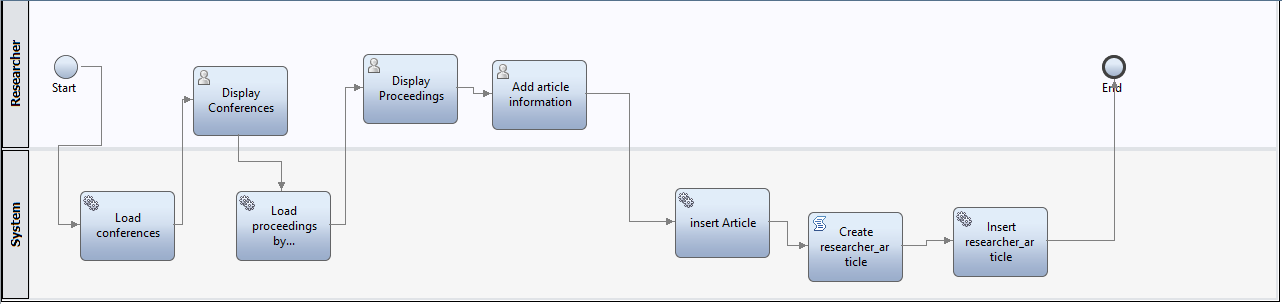
\includegraphics[scale=0.4]{diagrams/diagAddArticle.png} 
\caption{Diagram podprocesu pridania vedeckej publikácie}
\end{figure}

\subsubsection{Webová služba: Získanie všetkých vedeckých konferencií}
\textbf{Názov služby:} WS\_Conference\_findAll\\
\textbf{Metóda služby:} getAll\\
\textbf{Výstupy:}
	\begin{itemize}
		\item \textit{conferences} - list objektov typu Conference
	\end{itemize}
	
\subsubsection{Webová služba: Získanie zborníka podľa ľubovoľného atribútu}
\textbf{Názov služby:} WS\_Proceedings\_getByAttribute\\
\textbf{Metóda služby:} getByAttributeValue\\
\textbf{Vstupy:}
	\begin{itemize}
		\item \textit{attributes\_name} - názov atribútu
		\item \textit{attributes\_value} - hodnota atribútu
		\item \textit{listOf.Integer()} - zoznam ID zborníkov, z ktorých sa má hľadať, vytvárame nový prázdny list, aby metóda služby hľadala v celom rozsahu (všetkých IDs)
	\end{itemize}
\textbf{Výstupy:}
	\begin{itemize}
		\item \textit{proceedings} - list objektov typu Proceeding
	\end{itemize}
	
\subsubsection{Webová služba: Získanie zborníka podľa ľubovoľného atribútu}
\textbf{Názov služby:} WS\_Proceedings\_getByAttribute\\
\textbf{Metóda služby:} getByAttributeValue\\
\textbf{Vstupy:}
	\begin{itemize}
		\item \textit{attributes\_name} - názov atribútu
		\item \textit{attributes\_value} - hodnota atribútu
		\item \textit{listOf.Integer()} - zoznam ID zborníkov, z ktorých sa má hľadať, vytvárame nový prázdny list, aby metóda služby hľadala v celom rozsahu (všetkých IDs)
	\end{itemize}
\textbf{Výstupy:}
	\begin{itemize}
		\item \textit{proceedings} - list objektov typu Proceeding
	\end{itemize}
	
\subsubsection{Webová služba: Vloženie vedeckej publikácie}
\textbf{Názov služby:} WS\_Article\_insert\\
\textbf{Metóda služby:} insert\\
\textbf{Vstupy:}\\
	\begin{itemize}
		\item \textit{team\_id} - ID tímu, slúži na autentifikáciu webovej služby
		\item \textit{team\_password} - heslo, slúži na autentifikáciu webovej služby
		\item \textit{Article} - objekt typu Article s vyplnenými údajmi
	\end{itemize}
\textbf{Výstupy:}
	\begin{itemize}
		\item \textit{id} - ID novo vytvorenej vedeckej publikácie
	\end{itemize}
	
	\subsubsection{Skript: Pridaj nového spoluautora ku vedeckej publikácii}
Skript na vytvorenie nového objektu, ktorý priradí nového spoluautora k danej vedeckej publikácii. Potom tento objekt pridá webová služba do prepojovacej tabuľky Researcher\_Article.

\subsubsection{Webová služba: Vloženie entity spojovacej tabuľky Vedec - Publikácia}
\textbf{Názov služby:} WS\_Researcher\_article\_insert\\
\textbf{Metóda služby:} insert\\
\textbf{Vstupy:}
	\begin{itemize}
		\item \textit{team\_id} - ID tímu, slúži na autentifikáciu webovej služby
		\item \textit{team\_password} - heslo, slúži na autentifikáciu webovej služby
		\item \textit{researcher\_article} - objekt typu Researcher\_Article s vyplnenými údajmi
	\end{itemize}
\textbf{Výstupy:}
	\begin{itemize}
		\item \textit{id} - ID novo vytvorenej entity spojovacej tabuľky Vedec - Publikácia
	\end{itemize}

\section{Formuláre}
V tejto kapitole sú opísané všetky formuláre, ktoré nami implementované systémy používajú pri poskytovaní svojich funkcionalít.

\paragraph{Vybratie role}

\begin{figure} [H]
\centering

\includegraphics[scale=0.4]{forms/Coachforchoosingrole.png} 
\caption{Formulár pre vybratie role}
\end{figure}

V tomto formulári si používateľ vyberá či sa chce prihlásiť do systému ako výskumný pracovník alebo knihovník.

\paragraph{Prihlásenie používateľa}

\begin{figure} [H]
\centering
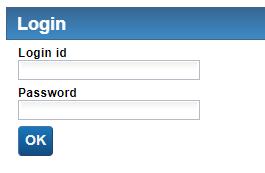
\includegraphics[scale=0.4]{forms/Coachforlogin.png} 
\caption{Formulár pre prihlásenie}
\end{figure}

Tento formulár slúži na prihásenie používateľa v akejkoľvek role (vedeckého pracovníka i knihovníka). Po kliknutí na tlačidlo OK dostane používateľ spatnú väzbu či bolo zadané heslo správne.

\paragraph{Výber akcie pridania publikácie alebo digitálneho objektu}

\begin{figure} [H]
\centering

\includegraphics[scale=0.4]{forms/Coachforresearchaction.png} 
\caption{Formulár pre výber akcie pridania publikácie alebo digitálneho objektu}
\end{figure}

Tento formulár slúži na výber akcie pre výskumníka, ktorý má dve možnosti buď pridať publikáciu, alebo pridať digitálny objekt k existujúcej publikácii.
Po vybraní príslučnej akcie sa výskumníkovi zobrazí príslušný formulár, ktorý s danou akciou súvisí.

\paragraph{Pridanie nového autora}

\begin{figure} [H]
\centering
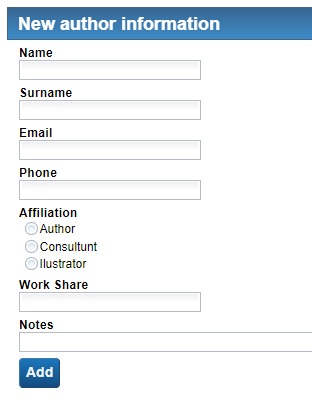
\includegraphics[scale=0.4]{forms/Coachforaddingnewauthor.png} 
\caption{Formulár pre pridanie nového autora}
\end{figure}

Tento formulár slúži na pridanie nového vedeckého pracovníka ako spolu-autora vedeckej publikácie. Tento formulár sa využíva pri pridávaní spolu-autorov k publikácií. Pridávaný vedecký pracovník sa uloží do databázy. Inštitúcia ku ktorej pracovník patrí je zvolená formulárom v jednom z predchádzajúcich krokov. O autorovi sú vyplnené nasledujúce údaje: meno, priezvisko, email, telefónne cislo, jeho afiliácia, podiel práce a poznámky k práci. Pridanie spolu-autora sa potvrdí kliknutím na tlačidlo Add.

\paragraph{Zobrazenie inštitúcií}

\begin{figure} [H]
\centering

\includegraphics[scale=0.4]{forms/CoachforDisplayInstitutions.png} 
\caption{Formulár pre zobrazenie inštitúcií}
\end{figure}

Tento formular slúži na výber inštitúcie z ktorej v neskoršom kroku pridáme spolu-autora k vedeckej publikácií. Vybrať je možné jednu inštitúciu z tabuľky a výber je potvrdený tlačidlom Choose.

\paragraph{Zobrazenie vedcov}

\begin{figure} [H]
\centering
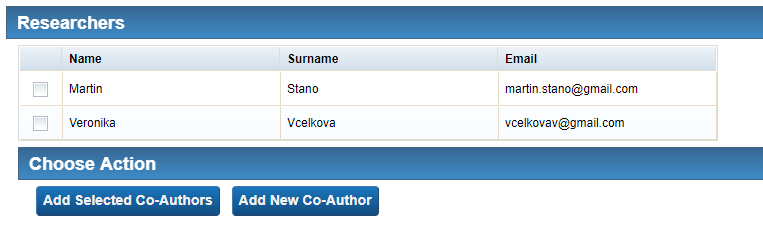
\includegraphics[scale=0.4]{forms/Coachfordisplayingresearchers.png} 
\caption{Formulár pre zobrazenie vedcov}
\end{figure}

V tomto formulári si používateľ môže zvoliť či chce pridať existujúcich vedeckých pracovníkov zo skôr vybranej inštitúcie ako spolu-autorov, alebo chce pridať nového autora. V prípade pridávania existujúcich spolu-autorov si používateľ vyberie jedného alebo viac vedeckých pracovníkov z tabuľky a výber potvrdí kliknutím na tlačidlo Add Selected Co-Authors. V prípade rozhodnutia pridať nového spolu-autora klikne používateľ na tlačidlo Add New Co-Author a bude presmerovaný na formulár New Author Information. 

\paragraph{Výber vedeckej publikácie}

\begin{figure} [H]
\centering
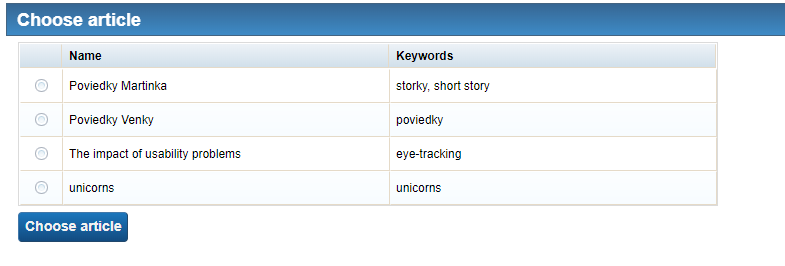
\includegraphics[scale=0.4]{forms/CoachChoosearticle.png} 
\caption{Formulár pre výber vedeckej publikácie}
\end{figure}

Tento formulár, ktorý je súčasťou knižničného informačného systému, slúži na výber vedeckého článku. Tieto články boli vyfiltrované, na základe zvoleného zborníku, ktoré boli rovnakým spôsobom filtorované zo zvolenej konferencie.

\paragraph{Výber vedeckej konferencie}

\begin{figure} [H]
\centering
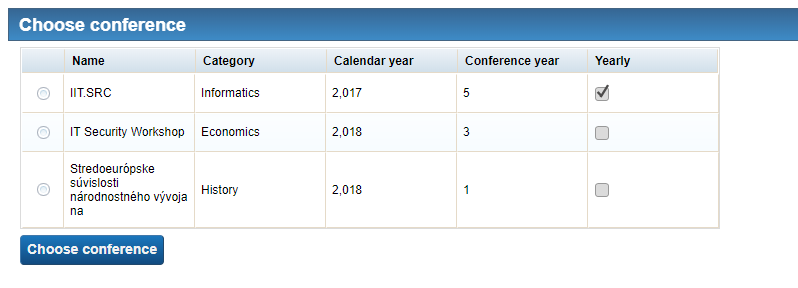
\includegraphics[scale=0.4]{forms/Coachchooseconference.png} 
\caption{Formulár pre výber vedeckej konferencie}
\end{figure}

Formulár slúži na výber konferencie zo zoznamu dostupných konferencií, čo v knižničnom informačnom systéme, ale aj v diginálnom repozitári, slúži k tomu, aby sa knihovník aj výskumník dostali k zborníkom, na základe zvolenej konferencie. To je potrebné pri viacerých biznis procesoch, ako napríklad: pridávanie digitálneho objektu ku konktétnemu článku, ktorý spadá pod zborník danej konferencie, ktorý môže pridať výskumník aj knihovník alebo pridávanie publikácie výskumníkom, ktorá sa opäť pridáva ku konkrétnemu zborníku vybranej konferencie.

\paragraph{Výber zborníku}

\begin{figure} [H]
\centering
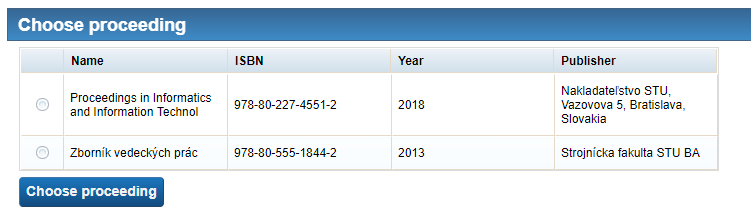
\includegraphics[scale=0.4]{forms/Choachchooseproceeding.png} 
\caption{Formulár pre výber zborníku}
\end{figure}

Výber zborníku, k čomu slúži tento formulár, nasleduje za výberom konferencie, na základe ktorej sa vyfiltrujú zborníky danej konferencie. Podobne ako výber konferencie aj výber zborníku sa nachádza v knižničnom ifnromačnom systéme aj digitálnom repozitári, nakoľko sa podieľa pri viacerých biznis procesoch.

\paragraph{Validovanie vedeckej publikácie}

\begin{figure} [H]
\centering
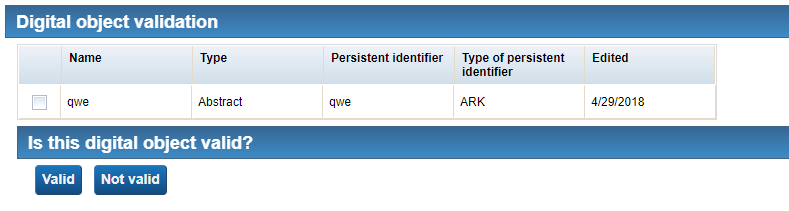
\includegraphics[scale=0.4]{forms/Coachforvalidatingpublication.png} 
\caption{Formulár pre validovanie vedeckej publikácie}
\end{figure}

Pointa formulára tkvie vo výbere diginálych objektov, ktoré chce knihovník označiť za validné, vrámci digitálneho repozitáru. Zo zoznamu vyfiltrovaných digitálnych objektov si vyberie jeden alebo viacero objektov, o ktorých validnosti chce rozhodnúť a následne vyberie príšlú akciu.

\paragraph{Možnosť pridania spoluautorov}

\begin{figure} [H]
\centering

\includegraphics[scale=0.4]{forms/Coachchoicetoaddcouthors.png} 
\caption{Formulár možnosti pridania spoluautorov}
\end{figure}

Formulár slúži na získanie rozhodnutia od výskumníka, ktorý buď chce, alebo nechce pridať spoluautorov vloženej publikácie, s ktorými sa pracuje v knižničnom informačnom systéme.

\paragraph{Pridanie digitálneho objektu}

\begin{figure} [H]
\centering
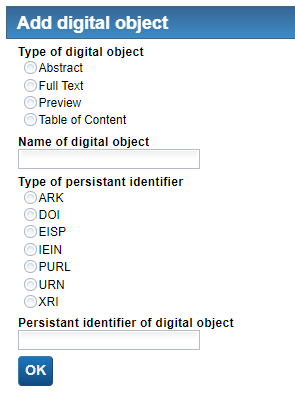
\includegraphics[scale=0.4]{forms/CoachforAdddigitalobject.png} 
\caption{Formulár pre pridanie digitálneho objektu}
\end{figure}

Tento formulár slúži na pridávanie digitálneho objektu (typu \textit{Digital{\_}object}) k existujúcej vedeckej publikácií (typu \textit{Article}). Digitálny objekt je pri tom uložení v digitálnom repozitáry. V tomto formuláry má používateľ možnosť si zvoliť typ digitálneho objektu (Abstract, Plný Text, Náhľad, Obsah), ktorý pridáva k publikácií. Následne zadá jeho názov a vyberie typ perzistentného identifikátora a zadá jeho adresu (hodnotu). Tlačidlom OK používateľ potvrdí pridanie digitálneho objektu.

\paragraph{Pridanie informácií o vedeckej publikácii}

\begin{figure} [H]
\centering
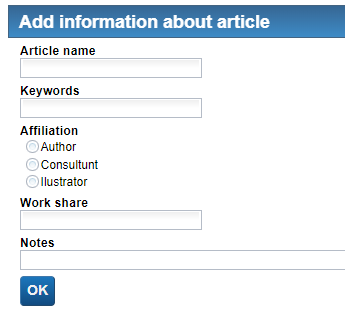
\includegraphics[scale=0.4]{forms/Coachforaddinginformationaboutarticle.png} 
\caption{Formulár pre pridanie informácií o vedeckej publikácii}
\end{figure}

Tento formulár slúži na pridanie novej vedeckej publikácie do knižničného informačného systému. Používateľ pri tomto procese zadá názov publikácie a jej kľúčové slová. Pridaním novej publikácie sa k nej zároveň ako prvý autor priradí práve prihlásený vedecký pracovník. Tým pádom je si nutné vybrať afiliáciu tohto autora, zadať jeho podieľ práce a prípadné poznámky k práci. Pridanie článku sa potvrdí kliknutím na tlačidlo OK.

\section{Prehľad všetkých webových služieb}
Z dôvodu prehľadnosti sme sa rozhodli zoskupiť všetky vyššie spomínané webové služby na jedno miesto.

\subsubsection{Webová služba: Získanie vedeckej publikácie}
\textbf{Názov služby:} WS\_Article\_find\\
\textbf{Metóda služby:} getById\\
\textbf{Vstupy:}\\
	\begin{itemize}
		\item \textit{id} - ID vedeckej publikácie
	\end{itemize}
\textbf{Výstupy:}
	\begin{itemize}
		\item \textit{article} - objekt typu Article
	\end{itemize}
	
\subsubsection{Webová služba: Získanie všetkých vedeckých publikácií}
\textbf{Názov služby:}  WS\_Article\_findAll\\
\textbf{Metóda služby:} getAll\\
\textbf{Výstupy:}\\
	\begin{itemize}
		\item \textit{articles} - list objektov typu Article
	\end{itemize}
	
\subsubsection{Webová služba: Získanie vedeckých publikácií na základe atribútu}
\textbf{Názov služby:} WS\_Article\_getByAttribute\\
\textbf{Metóda služby:} getByAttributeValue\\
\textbf{Vstupy:}\\
	\begin{itemize}
		\item \textit{attributes\_name} - názov atribútu
		\item \textit{attributes\_value} - hodnota atribútu
		\item \textit{listOf.Integer()} - zoznam ID vedeckých publikácií, z ktorých sa má hľadať, vytvárame nový prázdny list, aby metóda služby hľadala v celom rozsahu (všetkých IDs)
	\end{itemize}
\textbf{Výstupy:}
	\begin{itemize}
		\item \textit{articles} - list objektov typu Article
	\end{itemize}
	
\subsubsection{Webová služba: Vloženie vedeckej publikácie}
\textbf{Názov služby:} WS\_Article\_insert\\
\textbf{Metóda služby:} insert\\
\textbf{Vstupy:}\\
	\begin{itemize}
		\item \textit{team\_id} - ID tímu, slúži na autentifikáciu webovej služby
		\item \textit{team\_password} - heslo, slúži na autentifikáciu webovej služby
		\item \textit{Article} - objekt typu Article s vyplnenými údajmi
	\end{itemize}
\textbf{Výstupy:}
	\begin{itemize}
		\item \textit{id} - ID novo vytvorenej vedeckej publikácie
	\end{itemize}
	
\subsubsection{Webová služba: Telefonické notifikovanie}
\textbf{Názov služby:} WS\_Call\\
\textbf{Metóda služby:} notify\\
\textbf{Vstupy:}
	\begin{itemize}
		\item \textit{team\_id} - ID tímu, slúži na autentifikáciu webovej služby
		\item \textit{team\_password} - heslo, slúži na autentifikáciu webovej služby
		\item \textit{phone} - telefónne číslo, na ktoré sa má zatelefonovať
		\item \textit{"You were added as a coauthor"} - predmet správy, ktorá sa odošle
		\item \textit{"You are coauthor of article: " + tw.local.article\_id.toString()} - správa, ktorá sa telefonicky oznámi, kde article\_id.toString() predstavuje ID článku, ktorého je príjemca telefonátu spoluautorom
	\end{itemize}
\textbf{Výstupy:}
	\begin{itemize}
		\item \textit{success} - pravdivostná hodnota, ktorá vyjadruje, či sa podarilo telefonicky notifikovať spoluautora vedeckej publikácie
	\end{itemize}
	
\subsubsection{Webová služba: Získanie všetkých vedeckých konferencií}
\textbf{Názov služby:} WS\_Conference\_findAll\\
\textbf{Metóda služby:} getAll\\
\textbf{Výstupy:}
	\begin{itemize}
		\item \textit{conferences} - list objektov typu Conference
	\end{itemize}
	
\subsubsection{Webová služba: Vloženie vedeckej konferencie}
\textbf{Názov služby:} WS\_Conference\_insert\\
\textbf{Metóda služby:} insert\\
\textbf{Vstupy:}
	\begin{itemize}
		\item \textit{team\_id} - ID tímu, slúži na autentifikáciu webovej služby
		\item \textit{team\_password} - heslo, slúži na autentifikáciu webovej služby
		\item \textit{Conference} - objekt typu Conference s vyplnenými údajmi
	\end{itemize}
\textbf{Výstupy:}
	\begin{itemize}
		\item \textit{id} - ID novo vytvorenej vedeckej konferencie
	\end{itemize}
	
\subsubsection{Webová služba: Získanie všetkých digitálnych objektov}
\textbf{Názov služby:} WS\_Digital\_object\_findAll\\
\textbf{Metóda služby:} getAll\\
\textbf{Výstupy:}
	\begin{itemize}
		\item \textit{digital\_objects} - list objektov typu Digital\_object
	\end{itemize}
	
\subsubsection{Webová služba: Vloženie digitálneho objektu}
\textbf{Názov služby:} WS\_Digital\_object\_insert\\
\textbf{Metóda služby:} insert\\
\textbf{Vstupy:}
	\begin{itemize}
		\item \textit{team\_id} - ID tímu, slúži na autentifikáciu webovej služby
		\item \textit{team\_password} - heslo, slúži na autentifikáciu webovej služby
		\item \textit{digital\_object} - objekt typu Digital\_object s vyplnenými údajmi
	\end{itemize}
\textbf{Výstupy:}
	\begin{itemize}
		\item \textit{id} - ID novo vytvoreného digitálneho objektu
	\end{itemize}
	
\subsubsection{Webová služba: Aktualizovanie údajov digitálneho objektu}
\textbf{Názov služby:} WS\_Digital\_object\_update\\
\textbf{Metóda služby:} update\\
\textbf{Vstupy:}
	\begin{itemize}
		\item \textit{team\_id} - ID tímu, slúži na autentifikáciu webovej služby
		\item \textit{team\_password} - heslo, slúži na autentifikáciu webovej služby
		\item \textit{id} - ID digitálneho objektu, ktorý sa má aktualizovať
		\item \textit{digital\_object} - objekt typu Digital\_object s vyplnenými údajmi
	\end{itemize}
\textbf{Výstupy:}
	\begin{itemize}
		\item \textit{changes} - počet atribútov digitálneho objektu, ktoré sa aktualizovali
	\end{itemize}
	
\subsubsection{Webová služba: Získanie digitálneho objektu na základe ľubovoľného atribútu}
\textbf{Názov služby:} WS\_Digital\_objects\_getByAttibute\\
\textbf{Metóda služby:} getByAttributeValue\\
\textbf{Vstupy:}
	\begin{itemize}
		\item \textit{attribute} - názov atribútu, podľa ktorého sa má vyhľadávať
		\item \textit{value} - hodnota atribútu, podľa ktorého sa má vyhľadávať
		\item \textit{listOf.Integer()} - zoznam ID entít Vedec-Publikácia, z ktorých sa má hľadať, vytvárame nový prázdny list, aby metóda služby hľadala v celom rozsahu (všetkých IDs)
	\end{itemize}
\textbf{Výstupy:}
	\begin{itemize}
		\item \textit{digital\_objects\_array} - list objektov typu Digital\_object
	\end{itemize}
	
\subsubsection{Webová služba: Vloženie logovacieho záznamu}
\textbf{Názov služby:} WS\_Events\_insert\\
\textbf{Metóda služby:} insert\\
\textbf{Vstupy:}
	\begin{itemize}
		\item \textit{team\_id} - ID tímu, slúži na autentifikáciu webovej služby
		\item \textit{team\_password} - heslo, slúži na autentifikáciu webovej služby
		\item \textit{event} - objekt typu Events vyplnenými údajmi
	\end{itemize}
\textbf{Výstupy:}
	\begin{itemize}
		\item \textit{id} - ID novo vytvoreného logovacieho záznamu
	\end{itemize}
	
\subsubsection{Webová služba: Získanie všetkých inštitúcií}
\textbf{Názov služby:} WS\_Institution\_findAll\\
\textbf{Metóda služby:} getAll\\
\textbf{Výstupy:}
	\begin{itemize}
		\item \textit{institutions} - list objektov typu Institution
	\end{itemize}
	
\subsubsection{Webová služba: Vloženie inštitúcie}
\textbf{Názov služby:} WS\_Institution\_insert\\
\textbf{Metóda služby:} insert\\
\textbf{Vstupy:}
	\begin{itemize}
		\item \textit{team\_id} - ID tímu, slúži na autentifikáciu webovej služby
		\item \textit{team\_password} - heslo, slúži na autentifikáciu webovej služby
		\item \textit{institution} - objekt typu Institution s vyplnenými údajmi
	\end{itemize}
\textbf{Výstupy:}
	\begin{itemize}
		\item \textit{id} - ID novo vytvorenej inštitúcie
	\end{itemize}
	
\subsubsection{Webová služba: Získanie knihovníka}
\textbf{Názov služby:} WS\_Librarian\_find\\
\textbf{Metóda služby:} getById\\
\textbf{Vstupy:}
	\begin{itemize}
		\item \textit{id} - ID knihovníka
	\end{itemize}
\textbf{Výstupy:}
	\begin{itemize}
		\item \textit{librarian} - objekt typu Librarian
	\end{itemize}
	
\subsubsection{Webová služba: Získanie všetkých knihovníkov}
\textbf{Názov služby:} WS\_Librarian\_findAll\\
\textbf{Metóda služby:} getAll\\
\textbf{Výstupy:}
	\begin{itemize}
		\item \textit{librarians} - list objektov typu Librarian
	\end{itemize}
	
\subsubsection{Webová služba: Vloženie knihovníka}
\textbf{Názov služby:} WS\_Librarian\_insert\\
\textbf{Metóda služby:} insert\\
\textbf{Vstupy:}
	\begin{itemize}
		\item \textit{team\_id} - ID tímu, slúži na autentifikáciu webovej služby
		\item \textit{team\_password} - heslo, slúži na autentifikáciu webovej služby
		\item \textit{librarian} - objekt typu Librarian s vyplnenými údajmi
	\end{itemize}
\textbf{Výstupy:}
	\begin{itemize}
		\item \textit{id} - ID novo vytvoreného knihovníka
	\end{itemize}
	
\subsubsection{Webová služba: Získanie všetkých zborníkov}
\textbf{Názov služby:} WS\_Proceedings\_findAll\\
\textbf{Metóda služby:} getAll\\
\textbf{Výstupy:}
	\begin{itemize}
		\item \textit{proceedingss} - list objektov typu Proceedings
	\end{itemize}
	
\subsubsection{Webová služba: Získanie zborníka podľa ľubovoľného atribútu}
\textbf{Názov služby:} WS\_Proceedings\_getByAttribute\\
\textbf{Metóda služby:} getByAttributeValue\\
\textbf{Vstupy:}
	\begin{itemize}
		\item \textit{attributes\_name} - názov atribútu
		\item \textit{attributes\_value} - hodnota atribútu
		\item \textit{listOf.Integer()} - zoznam ID zborníkov, z ktorých sa má hľadať, vytvárame nový prázdny list, aby metóda služby hľadala v celom rozsahu (všetkých IDs)
	\end{itemize}
\textbf{Výstupy:}
	\begin{itemize}
		\item \textit{proceedings} - list objektov typu Proceeding
	\end{itemize}
	
\subsubsection{Webová služba: Získanie zborníka}
\textbf{Názov služby:} WS\_Proceedings\_getById\\
\textbf{Metóda služby:} getById\\
\textbf{Vstupy:}
	\begin{itemize}
		\item \textit{id} - ID zborníka
	\end{itemize}
\textbf{Výstupy:}
	\begin{itemize}
		\item \textit{proceedings} - objekt typu Proceedings
	\end{itemize}
	
\subsubsection{Webová služba: Vloženie zborníka}
\textbf{Názov služby:} WS\_Proceedings\_insert\\
\textbf{Metóda služby:} insert\\
\textbf{Vstupy:}
	\begin{itemize}
		\item \textit{team\_id} - ID tímu, slúži na autentifikáciu webovej služby
		\item \textit{team\_password} - heslo, slúži na autentifikáciu webovej služby
		\item \textit{proceedings} - objekt typu Proceedings s vyplnenými údajmi
	\end{itemize}
\textbf{Výstupy:}
	\begin{itemize}
		\item \textit{id} - ID novo vytvoreného zborníka
	\end{itemize}
	
\subsubsection{Webová služba: Aktualizovanie údajov zborníka}
\textbf{Názov služby:} WS\_Proceedings\_update\\
\textbf{Metóda služby:} update\\
\textbf{Vstupy:}
	\begin{itemize}
		\item \textit{team\_id} - ID tímu, slúži na autentifikáciu webovej služby
		\item \textit{team\_password} - heslo, slúži na autentifikáciu webovej služby
		\item \textit{id} - ID zborníka, ktorého údaje sa majú aktualizovať
		\item \textit{proceedings} - objekt typu Proceedings s vyplnenými údajmi
	\end{itemize}
\textbf{Výstupy:}
	\begin{itemize}
		\item \textit{changes} - počet atribútov digitálneho objektu, ktoré sa aktualizovali
	\end{itemize}
	
\subsubsection{Webová služba: Získanie všetkých entít spojovacej tabuľky Vedec-Publikácia}
\textbf{Názov služby:} WS\_Researcher\_Article\_getAll\\
\textbf{Metóda služby:} getAll\\
\textbf{Výstupy:}
	\begin{itemize}
		\item \textit{researcher\_articles} - list objektov typu Researcher\_Article
	\end{itemize}
	
\subsubsection{Webová služba: Získanie entity Vedec-Publikácia podľa ľubovoľného atribútu}
\textbf{Názov služby:} WS\_Researcher\_article\_getByAttribute\\
\textbf{Metóda služby:} getByAttributeValue\\
\textbf{Vstupy:}
	\begin{itemize}
		\item \textit{attribute\_name} - názov atribútu, podľa ktorého sa má vyhľadávať
		\item \textit{attribute\_value} - hodnota atribútu, podľa ktorého sa má vyhľadávať
		\item \textit{listOf.Integer()} - zoznam ID entít Vedec-Publikácia, z ktorých sa má hľadať, vytvárame nový prázdny list, aby metóda služby hľadala v celom rozsahu (všetkých IDs)
	\end{itemize}
\textbf{Výstupy:}
	\begin{itemize}
		\item \textit{researcher\_articles} - list objektov typu Researcher\_Article
	\end{itemize}
	
\subsubsection{Webová služba: Vloženie entity spojovacej tabuľky Vedec - Publikácia}
\textbf{Názov služby:} WS\_Researcher\_article\_insert\\
\textbf{Metóda služby:} insert\\
\textbf{Vstupy:}
	\begin{itemize}
		\item \textit{team\_id} - ID tímu, slúži na autentifikáciu webovej služby
		\item \textit{team\_password} - heslo, slúži na autentifikáciu webovej služby
		\item \textit{researcher\_article} - objekt typu Researcher\_Article s vyplnenými údajmi
	\end{itemize}
\textbf{Výstupy:}
	\begin{itemize}
		\item \textit{id} - ID novo vytvorenej entity spojovacej tabuľky Vedec - Publikácia
	\end{itemize}

\subsubsection{Webová služba: Získanie vedca}
\textbf{Názov služby:} WS\_Researcher\_find\\
\textbf{Metóda služby:} getById\\
\textbf{Vstupy:}
	\begin{itemize}
		\item \textit{id} - ID vedca
	\end{itemize}
\textbf{Výstupy:}
	\begin{itemize}
		\item \textit{researcher} - objekt typu Researcher
	\end{itemize}

\subsubsection{Webová služba: Získanie všetkých vedcov}
\textbf{Názov služby:} WS\_Researcher\_findAll\\
\textbf{Metóda služby:} getAll\\
\textbf{Výstupy:}
	\begin{itemize}
		\item \textit{researchers} - list objektov typu Researcher
	\end{itemize}
	
\subsubsection{Webová služba: Získaj vedca podľa ľubovoľného atribútu}
\textbf{Názov služby:} WS\_Researcher\_getByAttribute\\
\textbf{Metóda služby:} getByAttributeValue\\
\textbf{Vstupy:}
	\begin{itemize}
		\item \textit{name} - názov atribútu, podľa ktorého sa má vyhľadávať
		\item \textit{value} - hodnota atribútu, podľa ktorého sa má vyhľadávať
		\item \textit{listOf.Integer()} - zoznam ID vedcov, z ktorých sa má hľadať, vytvárame nový prázdny list, aby metóda služby hľadala v celom rozsahu (všetkých IDs)
	\end{itemize}
\textbf{Výstupy:}
	\begin{itemize}
		\item \textit{researchers} - list objektov typu Researcher 
	\end{itemize}
	
\subsubsection{Webová služba: Vloženie vedca}
\textbf{Názov služby:} WS\_Reasercher\_insert\\
\textbf{Metóda služby:} insert\\
\textbf{Vstupy:}
	\begin{itemize}
		\item \textit{team\_id} - ID tímu, slúži na autentifikáciu webovej služby
		\item \textit{team\_password} - heslo, slúži na autentifikáciu webovej služby
		\item \textit{researcher} - objekt typu Researcher s vyplnenými údajmi
	\end{itemize}
\textbf{Výstupy:}
	\begin{itemize}
		\item \textit{id} - ID novo vytvoreného vedca
	\end{itemize}
	
\subsubsection{Webová služba: Poslanie emailovej notifikácie}
\textbf{Názov služby:} WS\_Send\_email\\
\textbf{Metóda služby:} notify\\
\textbf{Vstupy:}
	\begin{itemize}
		\item \textit{team\_id} - ID tímu, slúži na autentifikáciu webovej služby
		\item \textit{team\_password} - heslo, slúži na autentifikáciu webovej služby
		\item \textit{email} - emailová adresa príjemcu notifikácie
		\item \textit{"You were added as a coauthor"} - predmet správy, ktorá sa odošle
		\item \textit{"Coauthor of article: " + tw.local.article\_id.toString()} - správa, ktorá sa odošle, kde article\_id.toString() predstavuje ID článku, ktorého je príjemca spoluautorom
	\end{itemize}
\textbf{Výstupy:}
	\begin{itemize}
		\item \textit{success} - pravdivostná hodnota, ktorá vyjadruje, či sa email podarilo odoslať
	\end{itemize}

\newpage

\section{Zhrnutie}
Táto práca je výsledkom analýzy získanej témy pre zadávanie bibliografických dokumentov a digitálnych objektov v systéme digitálneho repozitáru. Spracované sú biznis procesy, ktoré boli identifikované na základe zadania a následných konzultácií. Podobným spôsobom boli identifikované roly používateľov systému, ktoré majú rôzne práva. 

Navrhli sme dva systémy, ktoré spolu komunikujú - knižničný informačný systém a digitálny repozitár. Základom práce bolo navrhnúť proces a jeho podprocesy, ktoré predstavujú najpodstatnejšiu časť systému, a to pridanie článku, so všetkými atribútmi, ktoré ho definujú a pridanie a validovanie digitálneho objektu článku. Príkladom je náhľad alebo abstrakt konkrétneho bibliografického dokumentu. Spolu s tým boli definované jeho podprocesy spolu s formulármi, ktoré sú základom k implementovaniu funkcionality systému. Formuláre boli navrhnuté tak, aby boli čo najviac prehľadné, intuitívne a aby nimi boli zabezpečené správne entitno-relačné prepojenia v databáze, kde sme sa snažili vyhnúť zadávaniu id objektu, na ktorý má byť vytváraný objekt mapovaný. Riešením bolo ponúknuť používateľovi na výber z dostupných možností alebo ponúknutie vytvorenia objektu a jeho následné mapovanie.

Kvôli komplexnosti problémov vyplývajúcim zo zadania sa však používatelia prihlasujú práve pod spomínaným id a heslom, kde id poskytuje jednoznačný identifikátor, ktorý bolo vhodné použiť pri identifikácii.

V návrhu sú zahrnuté webové služby, najmä na notifikáciu používateľov ale i iné, súvisiace s databázou objektov a manipuláciou s nimi.

Návrhom sme sa snažili pokryť zadanie čo najlepšie, ako nám to dané prostriedky a webové služby dovoľovali.

\section{Report prác členov tímu}
\subsection{Dávid Kubík}
K vypracovaniu analýzy zadanej témy sme sa podielali v prvotných krokoch spoločne, kde sa definovali roly používateľov systému a entitno-relačný model. Potom sme prácu spracovávali paralelne v IBM Designer, pričom sme stále medzi sebou konzultovali nápady.  To zahŕňalo definovanie webových služieb a najmä tvorbu formulárov. Jedným z ďalších bodov, na ktorom som sa výrazne podielal, bolo tvorba dokumentácie k našej analýze, opísanie procesu, podprocesov, biznis objektov a celkovo fungovaniu návrhu.
\subsection{Martin Staňo}
K tomu, aby sme boli schopní vypracovať zadanie spoločne bez zbytočných nedorozumení sme zvolili prvotný brainstorming, kde sa definovali základné myšlienky, roly, procesy. Všetko sa konzultovalo až do bodu, kedy bola rozdelená ďalšia práca na projekte. V IBM som následne definoval základné služby, ktoré sme potrebovali k ďalšej práce a následne som pracoval na formulároch pre podprocesy a aj na samotných podprocesoch. Pri dokumentácii som prispel opisom vybraných podprocesov a pridaním screenshotov formulárov, ktoré v práci opisujeme.
\subsection{Veronika Včelková}
Náplň mojej práce spočívala v spoločnom prvotnom identifikovaní biznis objektov, ich prepojení a atribútov, rolí, ktoré vystupujú v systéme a náčrtu hlavného biznis procesu. Následne som sa zamerala na implementáciu v IBM Process Designer, kde som mala priradené webové služby vyplývajúce z objektov z nášho dátového modelu a následne priradené podprocesy definujúce hlavný biznis proces.

\end{document}